\chapterimage{BiosolidsRegulations.jpg} % Chapter heading image

\chapter{Biosolids Regulations}

\section{Biosolids Definition}\index{Biosolids Definition}

		\begin{itemize}
			\item Biosolids are treated solids produced as part of wastewater treatment
			\item Biosolids can be disposed or recycled beneficially
			\item Biosolids must meet standards established under Title 40 of the Code of Federal Regulations (CFR), Part 503.  
			\item Grit and screenings are not considered as biosolids
		\end{itemize}
	
\section{Biosolids Use/Disposal Methods}\index{Biosolids Use/Disposal Methods}
	
			\begin{enumerate}[1.]
				\item Land application
					\begin{itemize}
						\item This is the most commonly used biosolids management method and is referred as a "recycling" option.
						\item This uses the organic and/or nutrient content of the biosolids to either condition and/or fertilize crops or other vegetation grown in the soil
						\item Land application allows for the beneficial utilization of soil-enhancing constituents such as plant nutrients and organic matter in the biosolids
					\end{itemize}
				\item Surface disposal which requires availability of a large land which is lined with an impermeable material prior to the application of biosolids. 
				\item Incineration where the biosolids is burnt to ash.  This method utilizes its organic content to limit the amount of external fuel required to incinerate.  
			\end{enumerate}

\section{Biosolids Regulations}\index{Biosolids Regulations}

			\begin{itemize}
				\item Part 503 rule applies to any person who applies biosolids to the land or fires biosolids in a biosolids incinerator, and to the owner/operator of a surface disposal site, or to any person who is a preparer or generator of biosolids for use, incineration, or disposal.
				\item Part 503 standard includes:
					\begin{enumerate}
						\item General requirements
						\item Pollutant limits
						\item Management practices
						\item Operational standards, and
						\item Requirements for the frequency of monitoring, record-keeping, and reporting
					\end{enumerate}
			\end{itemize}



\section{Title 40 CFR Part 503 Requirements}\index{Title 40 CFR Part 503 Requirements}

In order to land apply biosolids, \underline{\emph{each} of the following three standards must be met}.

\subsection{Pollutant concentration limits}\index{Pollutant concentration limits}


			\begin{itemize}
				\item The biosolids produced must have concentrations of the 10 heavy metals listed, lower than the \texthl{Ceiling Concentration} thresholds.
				\item Sewage sludge exceeding the ceiling concentration limit for even one of the regulated pollutants is not classified as biosolids and, hence, cannot be land applied.
				\item Biosolids with heavy metal concentrations at or below the limit specified in the \texthl{Pollution Concentration} thresholds are classified as "High Quality Biosolids"
				\item Biosolids meeting pollutant concentration limits are subject to fewer requirements than biosolids meeting ceiling concentration limits
			\end{itemize}

\begin{figure}
	\begin{center}
		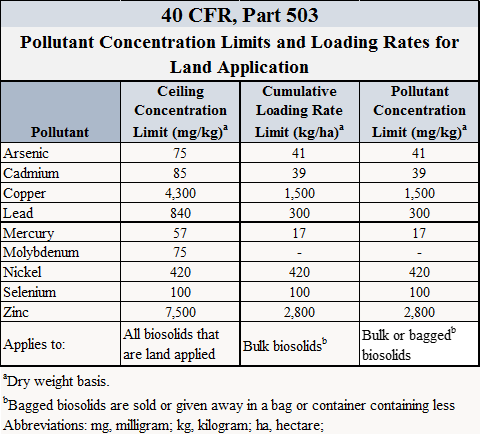
\includegraphics[scale=.82]{Table1}\\
			Table 5.1: Pollutant Concentration Limits and Loading Rates for Land Application
	\end{center}
	\end{figure}
\subsection{Pathogen reduction}\index{Pathogen reduction}
			\begin{itemize}
				\item Pathogens are disease causing organisms such as bacteria, viruses and parasites
				\item The treatment method used for treating wastewater solids must meet standards related to pathogen reduction
				\item Based upon the method used for treating wastewater solids, biosolids produced are classified as:
				\end{itemize}
\subsubsection{Class A Biosolids}\index{Class A Biosolids}
					\begin{itemize}
								\item The biosolids produced using the methods and standards identified are free of measurable pathogens.
								\item There are no pathogen related site restrictions for the application of Class A biosolids - including use in home gardens and landscaping
								\item Processes to further reduce pathogens \hl{(PFRP)} treatment, such as those involving high temperature, high pH with alkaline addition, drying, and composting, or their equivalent are most commonly used to demonstrate that biosolids meet Class A requirements
							\end{itemize}
\subsubsection{Class B Biosolids}\index{Class B Biosolids} 
									\begin{itemize}
										\item For Class B biosolids, pathogens have been reduced to levels that are unlikely to cause a threat to public health and the environment under specified use conditions.
										\item Processes to significantly reduce pathogens \hl{(PSRP)}, such as digestion, drying, heating, and high pH, or their equivalent are most commonly used to demonstrate that biosolids meet Class B requirements
										\item Site restrictions are imposed on the application of Class B biosolids to ensure minimizing the potential for human and animal contact with the biosolids until environmental factors reduce the pathogens to below detectable levels.
									\end{itemize}
\subsection{Vector attraction reduction}\index{Vector attraction reduction} 
			\begin{itemize}
				\item Vector reduction standards are for preventing transmission of pathogens via rodents, birds, and insects from the land applied biosolids.
				\item The vector reduction rule requirements are based on the following two approaches: 
					\begin{enumerate}
						\item Specifying organic matter decomposition processes viz., digestion and alkaline addition to mitigate vector attraction
						\item Biosolids sub-surface injection or incorporation within six hours so soil microbes out-competes/eliminates pathogens
					\end{enumerate}
				\item \hl{A minimum of 38\% volatile solids reduction} as part of the solids treatment process is a more common method of demonstrating compliance with vector attraction reduction requirements
			\end{itemize}
		\hl{For biosolids to qualify for Exceptional Quality (EQ) Standards - the application of which is almost unrestricted, it must meet all three of the following:}
		\begin{enumerate}
			\item Pollutant concentration limits
			\item Class A requirements
			\item Vector attraction reduction standards
		\end{enumerate}
		



\begin{sidewaysfigure}[!htp]
	\begin{center}
		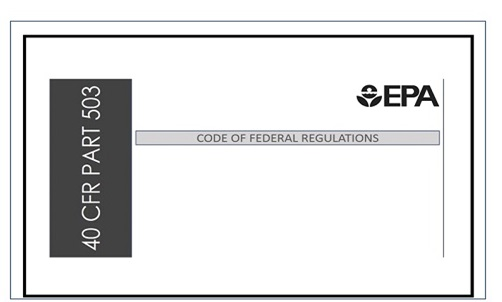
\includegraphics[scale=.55]{BiosolidsRegulations}
	\end{center}
\end{sidewaysfigure} 


\newpage
\section*{Chapter Assessment}
\begin{tcolorbox}[breakable, enhanced,
colframe=blue!25,
colback=blue!10,
coltitle=blue!20!black,  
title= Chapter Assessment]

\begin{enumerate}
\item  Grit and screenings from the preliminary treatment are also considered as biosolids \\

a. True \\
b. False \\

\item  A true statement regarding the term “biosolids” is: \\

a. The term is mandated for user by public law 92-500. \\
b. The term was developed by US EPA to define all biologically toxic precipitates. \\
c. The term is recommended by WEF for “a primarily organic solids product, produced by wastewater treatment processes, that can be beneficially recycled”. \\
d. The term is used by the California Water Resources Control Board to include “all insoluble matter derived from living aquatic organisms. \\

\item  When you spread sludge on agricultural land, the annual application rate of cadmium in the sludge should be less than 2 lbs/acre/year If your sludge contains 30 mg cadmium per kilogram of solids and your plant produces 950,000 lbs per year of dry solids, how many acres do you need? \\

a. 3 acres \\
b. 14 acres \\
c. 19 acres \\
d. 27 acres \\

\end{enumerate}
\end{tcolorbox}

